\documentclass[letter, 10pt]{article}
\usepackage[spanish]{babel}
\usepackage[utf8]{inputenc}
\usepackage{amsfonts}
\usepackage{amsmath}
\usepackage{graphicx}
\usepackage{url}
\usepackage[top=3cm,bottom=3cm,left=3.5cm,right=3.5cm,footskip=1.5cm,headheight=1.5cm,headsep=.5cm,textheight=3cm]{geometry}


\begin{document}
\title{Inteligencia Artificial \\ \begin{Large}Estado del Arte: Manejo de Trenes en Estaciones Ferroviarias\end{Large}}
\author{Martín Villanueva A.}
\date{23 de Mayo de 2016}
\maketitle


%--------------------No borrar esta secci\'on--------------------------------%
\section*{Evaluación}

\begin{tabular}{ll}
Resumen (5\%): & \underline{\hspace{2cm}} \\
Introducción (5\%):  & \underline{\hspace{2cm}} \\
Definición del Problema (10\%):  & \underline{\hspace{2cm}} \\
Estado del Arte (35\%):  & \underline{\hspace{2cm}} \\
Modelo Matemático (20\%): &  \underline{\hspace{2cm}}\\
Conclusiones (20\%): &  \underline{\hspace{2cm}}\\
Bibliografía (5\%): & \underline{\hspace{2cm}}\\
 &  \\
\textbf{Nota Final (100\%)}:   & \underline{\hspace{2cm}}
\end{tabular}
%---------------------------------------------------------------------------%
\vspace{2cm}


\begin{abstract}

\end{abstract}

\section{Introducción}


\section{Definición del Problema}
La definición del problema que se expone en esta sección, esta basada en \textit{ROADEF/Euro Challenge 2014} 
\cite{Problem}, con ciertas modificaciones y simplificaciones que se detallan en lo que sigue.


Como se mencionó anteriormente, el principal propósito del problema, consiste en encontrar la mejor
manera de manejar trenes en estaciones ferroviarias, entre las llegadas, las salidas y el uso de recursos
que hacen en la estación. Todo este proceso puede ser visto como una secuencia de subproblemas, sin embargo
aquí se trata y modela de una manera integrada. En vista de que el problema tiene en cuenta una gran 
cantidad de \textit{dimensiones}, a continuación se describen cada una de ellas de manera simple.

\begin{description}
	\item[\textsc{Horizonte de Planificación.}] 
	El horizonte de planificación corresponde al conjunto de instantes de tiempo (\textit{discretizados}),
	sobre el que se espera realizar toda la planificación del sistema. El formato de cada instante de tiempo
	es $(\text{d hh:mm:ss})$, con $\text{d } \in \{1, nbDays\}$ el día respectivo, $\text{hh } \in \{0,23\}$ 
	la hora, $\text{mm } \in \{0,59\}$ el minuto, y $\text{ss } \in \{0,59\}$ el segundo. El conjunto de todos
	los intantes se denominará $\mathcal{H}$. Con esta representación, el menor intervalo de tiempo permitido
	es un segundo, lo que permite representar el tiempo con una alta precisión. Sin embargo dependiendo de la 
	instancia, pueden tomarse duraciones más largas (múltiplos de segundos, o minutos), reduciendo el tamaño del
	\textit{espacio de búsqueda}.

	\item[\textsc{Llegadas.}]
	Las llegadas corresponden al ingreso de trenes en el sistema. Los tiempos de llegada (a la plataforma),
	son datos de entrada y por lo tanto no modificables. Hay que tomar en cuenta que los trenes entran al
	sistema/estación un tiempo antes que su hora de llegada. Durante este periodo intermedio realizan una
	\textit{secuencia de llegada}, que representan la secuencia de recursos (y los respectivos tiempos) de 
	los cuales hace uso el tren, antes de llegar a la plataforma para que los pasajeros bajen. Los aspectos
	y restricciones a considerar son los siguientes:
	\begin{enumerate}
		\item Cada llegada $a \in \mathcal{A}$ tiene un conjunto de plataformas preferidas a usar $\text{prefPlat}_a$.
		 Esta es una reestricción blanda, pero penalizada en la función objetivo.
		\item Existen tiempos ideal y máximo de permanencia en la plataforma: $\text{idealDwell}_a$ y $\text{maxDwell}_a$.
		Tiempos inferiores y superiores al $\text{idealDwell}_a$ son penalizados, pues el primero disminuye la satisfacción
		de los pasajeros que deben bajar, y el segundo constituye un mal uso de los recursos del sistema. En cualquier caso,
		el tiempo de permanencia no puede superar el máximo $\text{maxDwell}_a$.
		\item Es posible no cubrir una llegada, esto es, que el tren asociado a la llegada no entre a la estación. Como es de esperar, esto incurre una penalización.
	\end{enumerate}

	\item[\textsc{Salidas.}]
	Las salidas corresponden a la ida de trenes del sistema. Análogo a las entradas, los tiempos y secuencias de
	salida (ruteo entre los recursos hasta salir de la estación) son datos de entrada fijos. La principal tarea a
	cumplir aquí, es asignar un tren a cada salida. Los aspectos y restricciones a considerar son los siguientes:
	\begin{enumerate}
		\item No asignar un tren a un salida es penzalizado gravemente en la función objetivo. Adicionalmente, no
		puede asignarse más de un tren a un salida.
		\item Cada salida $d \in \mathcal{D}$ tiene un conjunto de plataformas preferidas a usar $\text{prefPlat}_d$.
		Esta es un reestricción blanda, pero penalizada en la función objetivo.
		\item Existen tiempos ideal y máximo de permanencia en la plataforma: $\text{idealDwell}_d$ y $\text{maxDwell}_d$.
		Las penalizaciones siguen la misma lógica que en las llegadas.
		\item Una salida tiene asociado un conjunto de categorías de trenes compatibles $\text{compCatDep}_d$. Esto va asociado a las características que debe tener el tren para hacer el viaje, y constituye una reestricción fuerte
		(no se puede violar).
		\item Cada tren tiene una \textit{distancia por recorrer antes de manteción} ($\text{remDBM}$) y \textit{tiempo de viaje antes de mantención} ($\text{remTBM}$). Cada salida tiene asociada un distancia y tiempo necesario para realizar el viaje. Luego el tren asignado debe tener $\text{remDBM}$ y $\text{remTBM}$ mayor o iguales a los que requiere la salida.

	\end{enumerate}

	\item[\textsc{Trenes.}]
	Un tren se define como una unidad movil de \textit{visita} en el sistema. Esto quiere decir que no se considera como tren
	a la unidad física; un mismo tren que visita más de una vez el sistema, se toma como trenes distintos. El conjunto de trenes $\mathcal{T}$ se compone de dos tipos de trenes: Los trenes presentes en la estación desde el inicio del horizonte de tiempo $\mathcal{T}_I$,  y los trenes asociados a llegadas $\mathcal{T}_A$.
	Las principales consideraciones a tener con los trenes son las siguientes:
	\begin{enumerate}
		\item Cada tren es una unidad atómica; No se pueden separar en vagones, ni recombinarlos con los de otros trenes. Por lo tanto un tren es la unidad de asignación más pequeñas. Como nota, esta reestricción es acorde a la naturaleza de los trenes modernos.
		\item Un tren $t \in \mathcal{T}$ esta asociado a una categoría $\text{cat}_t$, que define las características técnicas que comparten. Se puede pensar en los trenes de una misma categoría como el mismo tren (fabricado en serie por alguna compañia), pero con diferentes condiciones de mantención iniciales. 
		\item No ocupar los trenes inicialmente en el sistema es una opción posible, pero será penalizada. Tales trenes no usarán recursos durante el horizonte de planificación.
		\item Asociado una llegada y salida, puede haber un \textit{reuso}. Esto consiste en definir previamente (dato de entrada) cual tren que viene llegando, será asignado a una salida. Existe un costo asociado a no cumplir un reuso dado. Los reusos no serán respetados, siempre y caundo esto beneficie en mayor medida a otros objetivos. Por último,
		cada salida $d \in \mathcal{D}$ puede estar asociada a lo más en un reuso con la entrada $a \in \mathcal{A}$, y de igual modo al revés.
	\end{enumerate}

	\item[\textsc{Mantenciones.}]
	Los trenes deben ser sometidos a mantenciones regularmente, de modo que cumplan las condiciones de seguridad y comodidad necesarias que requiere cada salida. Cómo se mencionó anteriormente, hay dos parámetros a considerar en las manteciones:
	\begin{enumerate}
		\item \textbf{TBM}, el tiempo de viaje antes de realizar mantención (\textit{Time Before Maintanance}). Este va asociado al comodidad de los pasajeros (que el tren este limpio, asientos en buenas condiciones, etc).
		\item \textbf{DBM}, la distancia de viaje antes de realizar mantención (\textit{Distance Before Maintanance}). Se 
		relaciona con condiciones de seguridad (combustible, estado de frenos, etc).  
	\end{enumerate}
	Las operaciones de mantención básicamente reajustan los valores $\text{remTBM}$ y $\text{remDBM}$ a los valores máximos de cada tren. Las consideraciones a tener en cuenta son:
	\begin{enumerate}
		\item El movimiento de un tren dentro de la estación de resta a $\text{remTBM}$ y $\text{remDBM}$ (despreciables en comparación al de los viajes).
		\item Las mantenciones se realizan en las \textit{Instalaciones de Mantenimiento} descritas en la siguiente sección. 
	\end{enumerate}

	\item[\textsc{Recursos de Infraestructura.}]
	Los trenes en el sistema, estan siempre haciendo uso de algun recurso (ya sea moviendose o estacionados). Estos recursos
	son $5$ tipos: pistas simples $\mathcal{S}$, plataformas de llegada o salida $\mathcal{P}$, instalaciones de mantenimiento $\mathcal{F}$, grupos de pistas $\mathcal{K}$ y estacionamientos $\mathcal{Y}$. Las pistas simples, plataformas, y instalaciones de mantenimiento son consideradas como porciones individuales de una pista. Por otro lado 
	los grupos de pistas se constituyen de varias pistas de forma agregada. Una configuración típica para los recursos del
	sistema pueden verse en Figura \ref{fig:resources}.
 	\begin{figure}[htpb!]
	\centering
	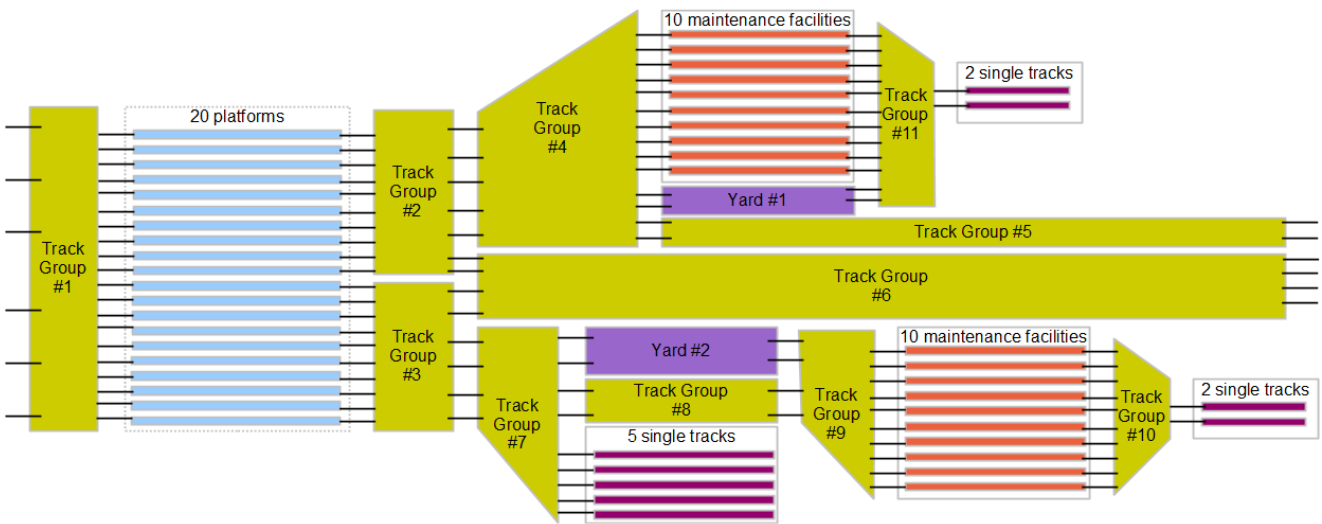
\includegraphics[width=12cm]{resources}
	\caption{Ejemplo de recursos de infraestructura (Fuente \cite{Problem})}
	\label{fig:resources}
	\end{figure}

	Es muy imporatente considerar la forma en que los trenes se mueven entre los recursos y sus restricciones. Los principales aspectos se listan como sigue:
	\begin{enumerate}
		\item Un mismo tren no puede estar ocupando dos recursos en el mismo instante de tiempo (algo que sí sucede en la realidad). Por lo tanto cada tren se considera como un objeto puntal que puede moverse de un recurso a otro de modo instantaneo.
		\item Cada recurso $r \in \mathcal{R}$ tiene un conjunto de recursos vecinos $\text{neighSet}_r$, que definen las posibles transiciones de un tren, esto es, un tren en un recurso $r$, sólo puede moverse a un recurso vecino en $\text{neighSet}_r$.
		\item Usualmente (hay excepciones) cada recurso puede ser accedido por dos lados, que se denotan A y B. Entonces el conjunto de recursos vecinos de $r$ puede ser descompuesto en $\text{neighSet}_r = \text{neighSet}_r^A \cup \text{neighSet}_r^B$. Adicionalmente se tiene como reestricción $\text{neighSet}_r^A \cap \text{neighSet}_r^B = \emptyset$, esto es, que no se generen ciclos entre los recursos.
		\item Las excepciones al punto anterior las constituyen los recursos al extremo del sistema, por donde los trenes entran o salen.
		\item Los recursos tienen en ambos extremos \textit{puertas} por donde se realiza la transición hacia otro recurso.
		Cada puerta $g \in \mathcal{G}_r$ de un recurso $r$, esta asociada a una única puerta de un recurso vecino (si la puerta esta en el fin del sistema, puede no tener puerta vecina asociada).
		\item Las pistas simples, plataformas y instalaciones de mantención tienen como máximo una puerta en cada lado.
		\item Los grupos de pistas y estacionamientos pueden tener mas de una puerta en cada lado. 
		\item Algunos recursos pueden ser utilizados sólo por un tipo específico de tren (por lo general en las estaciones de mantenimiento). Por ello cada recurso $r$ tiene su conjunto de categorías de trenes compatibles $\text{compCatRes}_r$.
		\item Pueden haber recursos ocupados con antelación en el sistema. Estos factores son externos al problema y fijos, siendo algunos ejemplos: trenes de mantenimiento, trenes que no terminan en la estación, trenes externos de otras compañias, entre otros. 
	\end{enumerate}

	Teniendo una idea de la mecánica de uso de recursos del sistema, a continuación se entregan detalles específicos de cada tipo de recurso.
	\begin{enumerate}
		\item \textbf{Pistas Simples.} Corresponden a pistas unitarias, usada para el movimiento de los trenes dentro de la estación. Estos son (usualmente) los recursos que utilizan los trenes para entrar y salir del sistema. Cada pista simple $s \in \mathcal{S}$ tiene asociado un largo total $\text{lenght}_s$ y cantidad de trenes $\text{capa}_s$,
		que debe ser respetado en cada instante de tiempo.
		\item \textbf{Plataformas.} Estas representan las pistas en donde los pasajeros pueden salir o abordar un tren. Por lo tanto son estas, las que deben ser asignadas a cada llegada o salida respectivo. A diferencia de las pistas simples, una plataforma $p \in \mathcal{P}$ sólo esta restrigida en capacidad por su largo $\text{lenght}_p$.
		\item \textbf{Instalaciones de Mantenimiento.} Estas instalaciones son pistas donde los trenes se detienen a realizar su respectiva mantención (reajustar su TBM y DBM). Es muy importante notar que cada instalación de mantenimiento $f \in \mathcal{F}$ esta equipada para hacer sólo un tipo de operación (``D'' o ``T''). Por lo tanto si un tren requiere hacer ambos mantenimientos, deberá pasar por dos instalaciones distintas. Por último, al igual que las plataformas, su capacidad esta restringida por su largo $\text{lenght}_f$.
		\item \textbf{Grupos de Pistas.} Son un conjunto agregado de pistas, utilizados para mover a los trenes entre los distintos recursos del sistema. Todas las puertas de un lado son alcanzables desde el otro (y viceversa), por lo tanto si en un lado hay $m$ puertas y en el otro lado hay $n$, existen $m\ n$ posibles rutas para atravesar el grupo de pistas. Un grupo de pistas $k \in \mathcal{K}$ tiene dos parámetros importantes: el tiempo necesario para atravesar $k$ $\text{trTime}_k$ (constante), y el tiempo mínimo que debe haber entre dos trenes sucesivos para que no esten tan cerca $\text{hwTime}_k$. Técnicamente los grupos de pistas son una estructura compleja, que debe manejar normas de seguridad y conflictos que suelen ocurrir. Sin embargo el problema se abstrae de esta complejidad, viendo a tal estructura como una \textit{caja negra}. 
		\item \textbf{Estacionamientos.} Al igual que el anterior, son también un conjunto de pistas pero utilizadas para estacionar trenes. Por lo tanto un tren puede permanecer en un estacionamiento sin limites de tiempo. Un estacionamiento $y \in \mathcal{Y}$ esta límitado en capacidad por la cantidad de trenes permitidos $\text{capa}_y$.
	\end{enumerate}


	\item[\textsc{Objetivo.}] Tal como se plantea el problema, la objetivo general se descompone en múltiples objetivos,
	que corresponden a minimizar las penalizaciones descritas anteriormente. Luego la función a minimizar es:
	\begin{align}
		f = f^{\text{uncov}} + f^{\text{over}} + f^{\text{plat}} + f^{\text{pref}} + f^{\text{reuse}},
		\label{eq:gobj}
	\end{align}
	donde cada una representa:
	\begin{enumerate}
		\item $f^{\text{uncov}}$: Costo por no cubrir una salida.
		\item $f^{\text{over}}$: Costo asociado al sobre-mantenimiento.
		\item $f^{\text{plat}}$: Costo por uso de las plataformas.
		\item $f^{\text{pref}}$: Costo por no respetar la preferencia de uso de plataforma.
		\item $f^{\text{reuse}}$: Costo por no respetar un reuso dado inicialmente. 
	\end{enumerate}
	un análisis más detallado de (\ref{eq:gobj}) será visto en la sección de Modelo Matemático.
	\item[\textsc{Solución Esperada.}] Como solución al problema, se espera una conjunto de programación de eventos
	para cada tren, esto es, una secuencia de eventos junto con los recursos usados, y los tiempos asociados. Los diferentes tipos de eventos pueden ser: \texttt{EnterSystem}, \texttt{ExitSystem}, \texttt{Arrival}, \texttt{Departure}, \texttt{EnterResource}, \texttt{ExitResource}, \texttt{BeginMaintenance} y \texttt{EndMaintenance}. Un ejemplo de posible solución para un tren dado se da en Figura \ref{fig:sched}.
	 \begin{figure}[htpb!]
	\centering
	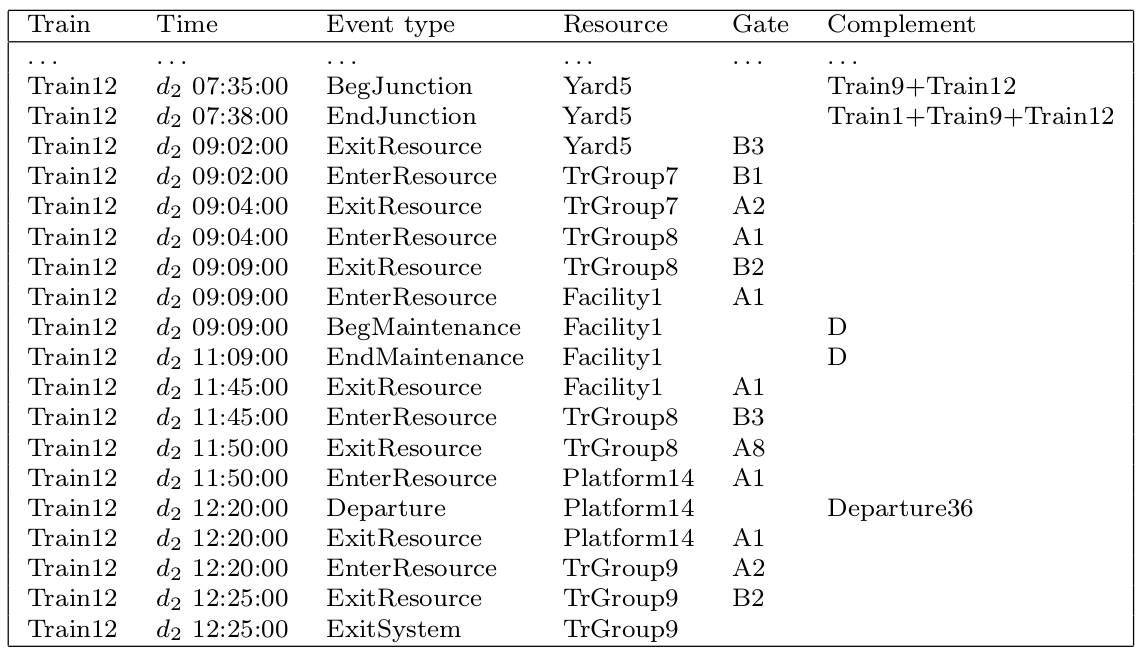
\includegraphics[width=12cm]{sched}
	\caption{Extracto de programación de eventos para un tren dado (Fuente \cite{Problem})}
	\label{fig:sched}
	\end{figure}
	Teniendo esta información para todos los trenes, sera posible inferir el estado del sistema y sus recursos, en cada instante del horizonte de planificación.

\end{description}


\section{Estado del Arte}


\section{Modelo Matemático}


\section{Conclusiones}


\section{Bibliografía}

\bibliographystyle{plain}
\bibliography{Referencias}

\end{document} 